\documentclass[conference]{IEEEtran}
\IEEEoverridecommandlockouts
% The preceding line is only needed to identify funding in the first footnote. If that is unneeded, please comment it out.
\usepackage{cite}
\usepackage{amsmath,amssymb,amsfonts}
\usepackage{algorithmic}
\usepackage{graphicx}
\usepackage{textcomp}
\usepackage{xcolor}
\usepackage{epstopdf}

\newcommand{\tabincell}[2]{\begin{tabular}{@{}#1@{}}#2\end{tabular}}
\def\BibTeX{{\rm B\kern-.05em{\sc i\kern-.025em b}\kern-.08em
    T\kern-.1667em\lower.7ex\hbox{E}\kern-.125emX}}
\begin{document}

\title{HTS:Research on Task Scheduling Technology for Heterogeneous Storage Media\\
{\footnotesize \textsuperscript{*}Note: Sub-titles are not captured in Xplore and
should not be used}
\thanks{Identify applicable funding agency here. If none, delete this.}
}

\author{\IEEEauthorblockN{1\textsuperscript{st} Given Name Surname}
\IEEEauthorblockA{\textit{dept. name of organization (of Aff.)} \\
\textit{name of organization (of Aff.)}\\
City, Country \\
email address}
\and
\IEEEauthorblockN{2\textsuperscript{nd} Given Name Surname}
\IEEEauthorblockA{\textit{dept. name of organization (of Aff.)} \\
\textit{name of organization (of Aff.)}\\
City, Country \\
email address}
\and
\IEEEauthorblockN{3\textsuperscript{rd} Given Name Surname}
\IEEEauthorblockA{\textit{dept. name of organization (of Aff.)} \\
\textit{name of organization (of Aff.)}\\
City, Country \\
email address}
\and
\IEEEauthorblockN{4\textsuperscript{th} Given Name Surname}
\IEEEauthorblockA{\textit{dept. name of organization (of Aff.)} \\
\textit{name of organization (of Aff.)}\\
City, Country \\
email address}
\and
\IEEEauthorblockN{5\textsuperscript{th} Given Name Surname}
\IEEEauthorblockA{\textit{dept. name of organization (of Aff.)} \\
\textit{name of organization (of Aff.)}\\
City, Country \\
email address}
\and
\IEEEauthorblockN{6\textsuperscript{th} Given Name Surname}
\IEEEauthorblockA{\textit{dept. name of organization (of Aff.)} \\
\textit{name of organization (of Aff.)}\\
City, Country \\
email address}
}

\maketitle

\begin{abstract}
In order to meet different workload demand, a large number of heterogeneous storage devices are usually deployed on each node in the data center, i.e. SSD and HDD. However, data processing frameworks such as MapReduce often considers that hardware is homogeneous and task scheduling is not aware of the difference between storage devices. In this case, if a large number of tasks are scheduled to low-speed storage nodes, it will greatly cause data processing bottlenecks. In this paper, we formulate Heterogeneous Storage-aware Task Scheduling Problem(HTS), and show its NP-hardness. In order to solve this problem, a stochastic algorithm is proposed, whose distance from the optimum value is within t with high probability. Experiments show that the algorithm can improve the performance of Hadoop default scheduling mechanism by 40\%.
\end{abstract}

\begin{IEEEkeywords}
big data, heterogeneous storage, task scheduling
\end{IEEEkeywords}

\section{Introduction}
This document is a model and instructions for \LaTeX.
Please observe the conference page limits. 

\section{RELATED WORKS}
The related works consist of two aspects. On the one hand, due to limited link bandwidth, some work is focused on data locality. On the other hand, in heterogeneous environments, it is not enough to consider data locality alone and some other studies have been carried out to accelerate data processing by studying hardware heterogeneity \cite{b1}.

Due to the limited network bandwidth resources in data center, if a large amount of data is transmitted between nodes during task execution, it will greatly affect the task performance. Therefore, processing data locally as much as possible can improve performance, i.e. placeing map task to the node which stores the input data. Matei et al. \cite{b2} proposes delay scheduling to assure data locality. Delay scheduling considers that when a node has idle slots, priority should be given to scheduling tasks with input data at that node, and delayed scheduling tasks without input data at that nodes. Ganesh \cite{b3} makes multiple replicas of high-frequency data by analyzing the access frequency of data, improve the data locality in this way. Cristina \cite{b4} proposes a distributed adaptive data replication algorithm DARE, which can help scheduler achieve better data locality. Jalaparti \cite{b5} believes that most of the production work is repetitive and predictable, which enables us to plan ahead. Coordinating and improving the tasks and data placement of these jobs can effectively reduce bandwidth usage and improve data locality. All of these work improves the performance of data processing by improving data locality.

However, in heterogeneous data centers, due to the different performance of data storage devices, task completion time is often different. At present, some of the existing work is based on the research of storage heterogeneity, which accelerates the method of large data processing. Xu et al. \cite{b6} considers the current usability of underlying hardware (CPU, memory, I/O), but does not consider the performance differences of different storage hardware. Pan et al. \cite{b7} takes into account the performance between different storage, but the problem can not be formally described. et al. Wang B \cite{b8} uses Markov model to describe the use of nodes in the cluster to deploy data reasonably. However, the scheduling problem of tasks is not considered, and the heterogeneity of different storage media is also not considered. These work does not accurately define the differences between storage hardwares, and choosing low-speed storage for a large amount of tasks can also lead to bottlenecks.

The difference between those tasks and ours are that our work clearly defines the difference in disk read speed and that deploying tasks according to different disk read speed to avoid bottlenecks.

\section{SYSTEM MODEL AND PROBLEM FORMULATION}
In this section, we first introduce the background of large data processing based on heterogeneous storage and build the system model. After that, the task scheduling problem with heterogeneous storage awareness is formulated as a  minimization problem whose objective is to minimize the maximum disk read time.

\subsection{Background and motivation}\label{AA}

A large number of query jobs are running on large data processing platforms, ie which have the requirements of low response lantacy and high quality of service. During execution, jobs are subdivided into tasks which scheduled to heterogeneous nodes. However, the general task scheduler i.e. FIFO scheduler is based on the fact that nodes are homogeneous, and the nodes with low computational power and high computational power will be deployed with the same amount of tasks. Tasks deployed by nodes with low computational power will have a longer execution time. The query job doesn't finish untill the completion of all tasks. Therefore, this kind of scheduling mechanism may cause the execution time of jobs to be too long to guarantee low query latency.

Task execution time is usually divided into two parts, one part is the lantacy of reading data from disk, the other part is the time of task execution in CPU. Experiments show that the reading time of low-speed disks can account for 70\% of the total task execution time, as shown in \ref{tab1}. Therefore, in order to ensure low latency of query jobs, data can be read from low $read-time$ disks. In the following section, we will use $read-time$ to represent the performance of a disk. This value is the time required to read a block from disk i.e. 64MB. The smaller the value, the better the disk performance. When reading N data from the disk, the total time is $read-time$ * N. In data centers, data is deployed in multiple copies on disks with different reading speeds. When data centers generate a large number of tasks, we consider deploying tasks to minimize the maximum disk $read-time$s,  thereby speeding up data processing.%tasks on high-speed disks and fewer tasks on low-speed disks to minimize the overall task's disk reading time, thereby speeding up large data processing.

\begin{table}[htbp]
	\caption{Comparisons of read time and execution time}
	\begin{center}
		\begin{tabular}{|c|c|c|c|}
			\hline
			\multicolumn{2}{|c|}{\textbf{The average value of 640MB data for  }} \\
			\hline
			\textbf{Read time(HDD)}& \textbf{Execution time (WordCount)}\\
			\hline
			3s & 1.5s  \\
			\hline
		\end{tabular}
		\label{tab1}
	\end{center}
\end{table}

As shown in Fig.\ref{fig1} there are four disks in the data center: DISK1, DISK2, DISK3 and DISK4. Each disk has different $read-time$, and $read-time$ of the four disks , $T$, are 0.3, 0.1, 0.2 and 0.2, respectively. The deployment of data replicas is shown in Fig.\ref{fig1}. When tasks are deployed, a general scheduler may place tasks such as scheduling1, and the execution time of the task is max \{$T_1 * N_1$, $T_2 * N_2$, $T_3 * N_3$,  $T_4 * N_4$, \} = max\{0.3*1, 0.1*1, 0.2*3, 0.2*1\}=0.3. Storage-aware task schedulers may place tasks as scheduling2, with a task execution time of at least 0.2. Obviously, the scheduling2 is optimum.

\begin{figure}[!t]
	\centering
	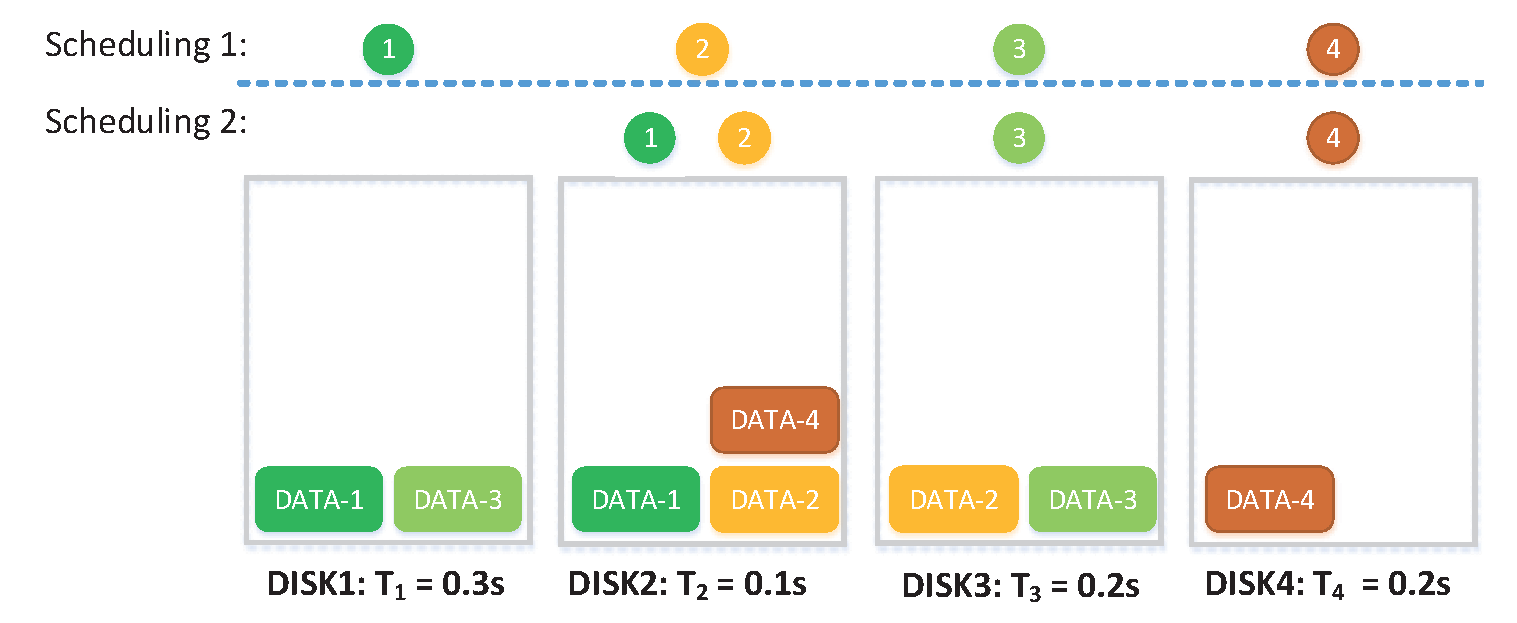
\includegraphics[height=1.5in]{fig1.eps}
	\caption{Comparison of task time between general task scheduling and disk-aware task scheduling. Scheduling1 is unaware of disk $read-time$ and the completion time of all tasks is max\{$T_1 * N_1$, $T_2 * N_2$, $T_3 * N_3$,  $T_4 * N_4$ \} = max\{0.3*1, 0.1*1, 0.2*3, 0.2*1\}= 0.3. Scheduling2 is aware of disk read time and the completion time of all tasks is max\{0, 0.1*2, 0.2*1, 0.2*1\} = 0.2. Scheduling2 is the optimum  \}
	\label{fig1}
\end{figure}

Example shows that when choosing the disk of the input data for a task, two things need to be considered: the first is the $read-time$ of a disk, and the second is the amount of tasks that are taking the data from the disk as input, that is, the load of the disk. These two things are able to ensure that there are no bottlenecks in the process of reading data from disk and the data processing can be accelerated.

\subsection{System Model}


\begin{table}[!t]
	\Large
	\centering
	\footnotesize
	\renewcommand\arraystretch{1.2}
	\caption{NOTATIONS USED IN THIS PAPER.}
	\label{table2}
	\begin{tabular}{c|l}
		\hline
		$\mathbb{D}$ & \tabincell{l}{The set of heterogeneous disks in datacenter} \\
		\hline
		 $\mathcal{M}$ & \tabincell{l}{The set of data in datacenter} \\
		\hline
		$\mathbb{T}$ & \tabincell{l}{The set of tasks to be scheduled} \\
		\hline
		$d_{i}$ & \tabincell{l}{The disk $i$ and $d_i \in \mathbb{D}$ } \\
		\hline
		$t_{j}$ & \tabincell{l}{The task $j$ and $t_j \in \mathbb{T}$ } \\
		\hline
		$m_{l}$ & \tabincell{l}{The data $l$ and $m_j \in \mathbb{M}$ } \\
		\hline
		$r_{l}^{k}$ & \tabincell{l}{The data replica $k$ of data  $m_l $ } \\
		\hline
		$read-time$ & \tabincell{l}{This time of reading a data block from disk } \\
		\hline
		$T_{i}$ & \tabincell{l}{The read-time of disk $d_i$} \\
		\hline	
		${I}_i^j$ & \tabincell{l}{A binary variable indicating if task $t_{i}$ choose the replica \\ that stored in $d_{i}$ as input  or not}\\
		\hline
		$\phi(t_j)$ & The data that task $t_j$ needs, and $\phi(t_j)$ $\in$  $\mathcal{M}$ \\
		\hline
		$\pi_{l}^{i}$ & \tabincell{l}{A binary variable indicating if data $m_l$ are \\stored at disk $d_i$ or not} \\
		\hline
		$h_{ul}$, $h_{dl}$ & \tabincell{l}{the channel fading coefficient for uplink and downlink} \\
		\hline
		$\phi(t_j)$ & The data that task $t_j$ needs \\
		\hline\\
		$N_(i)$ & Number of tasks which select data from disk i as input \\
		\hline
 \end{tabular}
\end{table}

\subsection{Heterogeneous Storage-aware Task Scheduling Problem (HTS)}
Number equations consecutively. To make your 
equations more compact, you may use the solidus (~/~), the exp function, or 
appropriate exponents. Italicize Roman symbols for quantities and variables, 
but not Greek symbols. Use a long dash rather than a hyphen for a minus 
sign. Punctuate equations with commas or periods when they are part of a 
sentence, as in:
\begin{equation}
a+b=\gamma\label{eq}
\end{equation}

Be sure that the 
symbols in your equation have been defined before or immediately following 
the equation. Use ``\eqref{eq}'', not ``Eq.~\eqref{eq}'' or ``equation \eqref{eq}'', except at 
the beginning of a sentence: ``Equation \eqref{eq} is . . .''

\section{PERFORMANCE EVALUATION}


\subsection{Simulation Settings}\label{SCM}
\begin{itemize}
\item The word ``data'' is plural, not singular.

\end{itemize}
An excellent style manual for science writers is \cite{b7}.

\subsection{Simulation Results}
\textbf{The class file is designed for, but not limited to, six authors.} A 
minimum of one author is required for all conference articles. Author names 
should be listed starting from left to right and then moving down to the 
next line. This is the author sequence that will be used in future citations 
and by indexing services. Names should not be listed in columns nor group by 
affiliation. Please keep your affiliations as succinct as possible (for 
example, do not differentiate among departments of the same organization).


\subsection{Figures and Tables}
\paragraph{Positioning Figures and Tables} Place figures and tables at the top and 
bottom of columns. Avoid placing them in the middle of columns. Large 
figures and tables may span across both columns. Figure captions should be 
below the figures; table heads should appear above the tables. Insert 
figures and tables after they are cited in the text. Use the abbreviation 
``Fig.~\ref{fig}'', even at the beginning of a sentence.



Figure Labels: Use 8 point Times New Roman for Figure labels. Use words 
rather than symbols or abbreviations when writing Figure axis labels to 
avoid confusing the reader. As an example, write the quantity 
``Magnetization'', or ``Magnetization, M'', not just ``M''. If including 
units in the label, present them within parentheses. Do not label axes only 
with units. In the example, write ``Magnetization (A/m)'' or ``Magnetization 
\{A[m(1)]\}'', not just ``A/m''. Do not label axes with a ratio of 
quantities and units. For example, write ``Temperature (K)'', not 
``Temperature/K''.


\begin{table}[htbp]
	\caption{Comparisons of read time and execution time}
	\begin{center}
		\begin{tabular}{|c|c|c|c|}
			\hline
			\textbf{Table}&\multicolumn{3}{|c|}{\textbf{Table Column Head}} \\
			\cline{2-4} 
			\textbf{Head} & \textbf{\textit{Table column subhead}}& \textbf{\textit{Subhead}}& \textbf{\textit{Subhead}} \\
			\hline
			copy& More table copy$^{\mathrm{a}}$& &  \\
			\hline
			\multicolumn{4}{l}{$^{\mathrm{a}}$Sample of a Table footnote.}
		\end{tabular}
		\label{tab1}
	\end{center}
\end{table}


\section{CONCLUSION}

\section*{Acknowledgment}

The preferred spelling of the word ``acknowledgment'' in America is without 
an ``e'' after the ``g''. Avoid the stilted expression ``one of us (R. B. 
G.) thanks $\ldots$''. Instead, try ``R. B. G. thanks$\ldots$''. Put sponsor 
acknowledgments in the unnumbered footnote on the first page.

\section*{References}

Please number citations consecutively within brackets \cite{b1}. The 
sentence punctuation follows the bracket \cite{b2}. Refer simply to the reference 
number, as in \cite{b3}---do not use ``Ref. \cite{b3}'' or ``reference \cite{b3}'' except at 
the beginning of a sentence: ``Reference \cite{b3} was the first $\ldots$''

Number footnotes separately in superscripts. Place the actual footnote at 
the bottom of the column in which it was cited. Do not put footnotes in the 
abstract or reference list. Use letters for table footnotes.

Unless there are six authors or more give all authors' names; do not use 
``et al.''. Papers that have not been published, even if they have been 
submitted for publication, should be cited as ``unpublished'' \cite{b4}. Papers 
that have been accepted for publication should be cited as ``in press'' \cite{b5}. 
Capitalize only the first word in a paper title, except for proper nouns and 
element symbols.

For papers published in translation journals, please give the English 
citation first, followed by the original foreign-language citation \cite{b6}.

\begin{thebibliography}{00}
\bibitem{b1} Ahmad F, Chakradhar S T, Raghunathan A, et al. Tarazu: optimizing mapreduce on heterogeneous clusters[C]//ACM SIGARCH Computer Architecture News. ACM, 2012, 40(1): 61-74.
\bibitem{b2} Zaharia M, Borthakur D, Sen Sarma J, et al. Delay scheduling: a simple technique for achieving locality and fairness in cluster scheduling[C]//Proceedings of the 5th European conference on Computer systems. ACM, 2010: 265-278.
\bibitem{b3} Ananthanarayanan G, Agarwal S, Kandula S, et al. Scarlett: coping with skewed content popularity in mapreduce clusters[C]//Proceedings of the sixth conference on Computer systems. ACM, 2011: 287-300.
\bibitem{b4} Abad C L, Lu Y, Campbell R H. DARE: Adaptive data replication for efficient cluster scheduling[C]//2011 IEEE international conference on cluster computing. IEEE, 2011: 159-168.
\bibitem{b5} Jalaparti V, Bodik P, Menache I, et al. Network-aware scheduling for data-parallel jobs: Plan when you can[C]//ACM SIGCOMM Computer Communication Review. ACM, 2015, 45(4): 407-420.
\bibitem{b6} Xu L, Butt A R, Lim S H, et al. A heterogeneity-aware task scheduler for spark[C]//2018 IEEE International Conference on Cluster Computing (CLUSTER). IEEE, 2018: 245-256.
\bibitem{b7} Pan F, Xiong J, Shen Y, et al. H-Scheduler: Storage-Aware Task Scheduling for Heterogeneous-Storage Spark Clusters[C]//2018 IEEE 24th International Conference on Parallel and Distributed Systems (ICPADS). IEEE, 2018: 1-9.
\bibitem{b8} Wang B, Jiang J, Yang G. Actcap: Accelerating mapreduce on heterogeneous clusters with capability-aware data placement[C]//2015 IEEE Conference on Computer Communications (INFOCOM). IEEE, 2015: 1328-1336
\end{thebibliography}
\end{document}
